\section{Fourier Transforms} \label{sec:fourier}

\subsection{Eigenfunctions and $H(s)$}

An \emph{eigenfunction} $x(t) = e^{j\omega t}$ is a function such that
$S\{x(t)\} = Ax(t)$ for LTI $S$. A property of functions of the form
$e^{j\omega t}$ is that convolution with $h(t)$ yields
\begin{equation}
    x(t) * h(t) = e^{j\omega t} \int_{-\infty}^{\infty} h(\tau) e^{-j\omega \tau} d\tau.
\end{equation}
This is also written as
\begin{equation}
    x(t) * h(t) = e^{j\omega t} \left( |H(j\omega)|e^{j \angle H(j\omega)} \right)
\end{equation}
$H$ is known as the transfer function as has the property that
$Y(S) = H(s)X(s)$, where $Y(s)$ and $X(s)$ are the Laplace transforms
of $y(t)$ and $x(t)$.

\section{Fourier Series}

Throughout this class we will sometimes see the expression $X(j\omega)$
or $X(e^{j\omega})$.
Note that these are defined as
\begin{equation}
    X(j\omega) = \int_{-\infty}^{\infty} x(t) e^{-j\omega t} dt
\end{equation}
for CT and
\begin{equation}
    X(e^{j\omega}) = \sum_{n=-\infty}^{\infty} x[n] e^{-j\omega n}
\end{equation}

A signal $x(t)$ is well-behaved iff
\begin{itemize}
    \item $x(t)$ is absolutely integrable over its domain.
    \item $x(t)$ has finite maximum and minimum.
    \item $x(t)$ has finite discontinuities.
\end{itemize}

\subsection{Continuous Time}

Consider an arbitrary periodic CT signal $x(t)$ with fundemental
period $T$ and fundemental frequency $\omega_0$. The Fourier series
representation of $x(t)$ is
\begin{align}\label{eq:synthesis}
    x(t) & = \sum_{k=-\infty}^{\infty} a_k e^{jk\omega_0 t}                                  \\
         & = a_0 + a_1e^{j\omega_0 t} + a_{-1}e^{-j\omega_0 t} + a_2e^{2j\omega_0 t} + \dots
\end{align}
where $a_k$ is the $k$th Fourier coefficient and can be found with the formula
\begin{equation}
    a_k = \frac{1}{T} \int_{<T>} x(t) e^{-jk\omega_0 t} dt
\end{equation}
with $<T>: [0, T], [-\frac{T}{2}, \frac{T}{2}, ...]$.
Equation \ref{eq:synthesis} is known as the synthesis equation. The process of
of finding $a_k$ is Fourier analysis.

Notably, $a_0$ gives the DC component of the signal. In general the $a_{\pm k}$
are the $k$th harmonic components.

Let's see an example. Let $x(t)$ be a square wave given by
\begin{equation}
    x(t) = \begin{cases}
        1 & |t| < T_1               \\
        0 & T_1 < |t| < \frac{T}{2}
    \end{cases}
\end{equation}

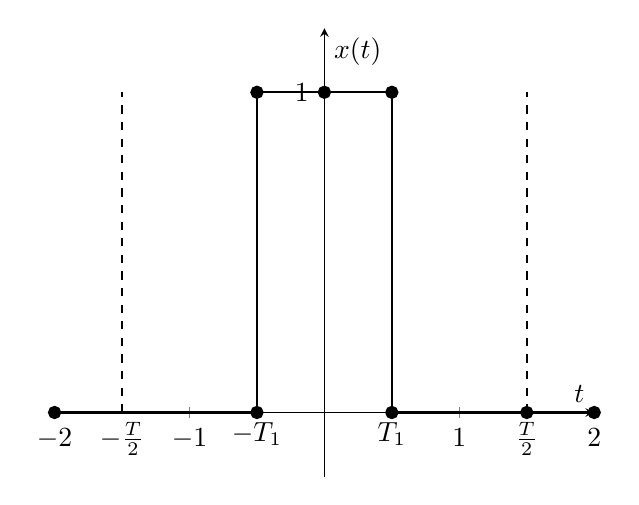
\begin{tikzpicture}
    \begin{axis}[
            axis x line=middle,
            axis y line=middle,
            xlabel={$t$},
            ylabel={$x(t)$},
            xtick={-2, -1, 0, 1, 2},
            ytick={0, 1},
            ymin=-0.2, ymax=1.2,
            xmin=-2, xmax=2,
            samples=100,
            domain=-2:2,
        ]
        \addplot[
            domain=-2:2,
            samples at={-2,-1.5,-1, -0.5, 0, 0.5, 1, 1.5, 2},
            mark=*,
            thick
        ] coordinates {(-2,0) (-0.5,0) (-0.5,1) (0,1) (0.5,1) (0.5,0) (1.5,0) (2,0)};

        \addplot[dashed, thick] coordinates {(-0.5,0) (-0.5,1)};
        \addplot[dashed, thick] coordinates {(0.5,0) (0.5,1)};
        \addplot[dashed, thick] coordinates {(1.5,0) (1.5,1)};
        \addplot[dashed, thick] coordinates {(-1.5,0) (-1.5,1)};

        \node[anchor=north] at (axis cs:-0.5,0) {$-T_1$};
        \node[anchor=north] at (axis cs:0.5,0) {$T_1$};
        \node[anchor=north] at (axis cs:1.5,0) {$\frac{T}{2}$};
        \node[anchor=north] at (axis cs:-1.5,0) {$-\frac{T}{2}$};
    \end{axis}
\end{tikzpicture}

We calculate $a_k$ as
\begin{align}
    a_k & = \frac{1}{T} \int_{<T>} x(t) e^{-jk\omega_0 t} dt                                         \\
        & = -\frac{1}{jk\omega_0 T} \left[ e^{-jk\omega_0 T_1} -  e^{jk\omega_0 T_1}\right]          \\
        & = \frac{1}{k\omega_0 T} \left[ \frac{e^{jk\omega_0 T_1} -  e^{-jk\omega_0 T_1}}{j} \right] \\
        & = \frac{2}{\omega_0 T} \sin(k \omega_0 T_1)                                                \\
        & = \frac{1}{\pi k} \sin(k \omega_0 T_1)
\end{align}
This expression for $a_0$ is fine, however, there is a problem. When
$k = 0$ we have a discontinuity. In general we may have to find $a_0$
separately. It's not a big deal: $a_0 = \frac{1}{T} \int_{-T_1}^{T_1} x(t) dt$ in general`'.

\subsection{Discrete Time}

In discrete time, an arbitrary periodic signal $x[n]$ with fundemental
period $N$ and fundemental frequency $\omega_0$. The Fourier series
representation of $x[n]$ is
\begin{align}\label{eq:dtsynthesis}
    x[n] & = \sum_{k=<N>} a_k x_k[n]           \\
         & = \sum_{k=<N>} a_k e^{jk\omega_0 n}
\end{align}

This expression yields a system of $n$ linear equations with $n$
unknowns, namely $x[0]$, $x[1]$, $\dots$, $x[n]$. In theory we
could solve this, perhaps using computers or linear algebra, but
in practice there is a simpler way. Multiply equation \ref{eq:dtsynthesis}
by $e^{-jr\frac{2\pi}{N}n}$ for any $r$ and sum over $N$ terms. Then
\begin{equation}
    \sum_{n=<N>} x_k[n] e^{-jr\frac{2\pi}{N}n} = \sum_{n=<N>} a_k \sum_{n=<N>} e^{j(k-r)(\frac{2\pi}{N})n}.
\end{equation}
Solving for $a_k$,
\begin{equation}
    a_k = \frac{1}{N} \sum_{n=<N>} x[n] e^{-jk\frac{2\pi}{N}n},
\end{equation}
which is the synthesis equation in discrete time.

A fun property is that $a_{k+N} = a_k$, so $a_k$ are periodic in $N$.

\subsection{Spectrum Analysis}

$a_k$ as a function of $k$ given the \emph{spectrum} of $x(t)$. Let's see
an example: let $T_1 = \frac{T}{4}$. Then $a_k = \frac{\sin(\pi \frac{k}{2})}{k\pi}$.

\begin{tikzpicture}
    \begin{axis}[
            axis x line=middle,
            axis y line=middle,
            xlabel={$t$},
            ylabel={$x(t)$},
            xtick={-2, -1, 0, 1, 2},
            ytick={0, 1},
            ymin=-0.2, ymax=1.2,
            xmin=-2, xmax=2,
            samples=100,
            domain=-2:2,
        ]
        \addplot[
            domain=-2:2,
            samples at={-2,-1.5,-1, -0.5, 0, 0.5, 1, 1.5, 2},
            only marks
        ] coordinates {((0,0.5) ((1,0.32) (-1, 0.32) (-2,0) (3, -0.1) (-3, -0.1) };
    \end{axis}
\end{tikzpicture}

\subsection{Properties}

Some useful properties follow from the definition
of the Fourier series.

\begin{table}[ht]
    \centering
    \label{tab:ctfourier_properties}
    \begin{tabular}{llll}
        \toprule
        \textbf{Property}    & \textbf{Time Domain}             &                                 & \textbf{Frequency Domain}                 \\
        \midrule
        Linearity            & $A x_1(t) + B x_2(t)$            & $\overset{FS}{\leftrightarrow}$ & $A a_k + B b_k$                           \\
        Even Symmetry        & $x(t)$ even                      & $\overset{FS}{\leftrightarrow}$ & $a_k$ even                                \\
        Odd Symmetry         & $x(t)$ odd                       & $\overset{FS}{\leftrightarrow}$ & $a_k$ odd                                 \\
        Time Shifting        & $x(t - t_0)$                     & $\overset{FS}{\leftrightarrow}$ & $a_k e^{-j k \omega_0 t_0}$               \\
        Frequency Shifting   & $x(t) e^{j n \omega_0 t}$        & $\overset{FS}{\leftrightarrow}$ & $a_{k - n}$                               \\
        Time Reversal        & $x(-t)$                          & $\overset{FS}{\leftrightarrow}$ & $a_{-k}$                                  \\
        Conjugation          & $x^*(t)$                         & $\overset{FS}{\leftrightarrow}$ & $a_{-k}^*$                                \\
        Periodic Convolution & $(x \ast y)(t)$                  & $\overset{FS}{\leftrightarrow}$ & $a_k b_k$                                 \\
        Multiplication       & $x(t) y(t)$                      & $\overset{FS}{\leftrightarrow}$ & $\sum_{n=-\infty}^{\infty} a_n b_{k - n}$ \\
        Differentiation      & $\frac{d}{dt} x(t)$              & $\overset{FS}{\leftrightarrow}$ & $j k \omega_0 a_k$                        \\
        Integration          & $\int x(t) dt$                   & $\overset{FS}{\leftrightarrow}$ & $\frac{a_k}{j k \omega_0}$ if $a_0 = 0$)  \\
        Parseval's Theorem   & $\frac{1}{T} \int_T |x(t)|^2 dt$ & $\overset{FS}{\leftrightarrow}$ & $\sum_{k=-\infty}^{\infty} |a_k|^2$       \\
        \bottomrule
    \end{tabular}
\end{table}

\begin{table}[ht]
    \centering
    6    \label{tab:dtfourier_properties}
    \begin{tabular}{llll}
        \toprule
        \textbf{Property}    & \textbf{Time Domain}                    &                                     & \textbf{Frequency Domain}                                       \\
        \midrule
        Linearity            & \(A\,x_1[n] + B\,x_2[n]\)               & \(\overset{DTFS}{\leftrightarrow}\) & \(A\,a_k + B\,b_k\)                                             \\
        Even Symmetry        & \(x[n]\) even (i.e., \(x[n]=x[-n]\))    & \(\overset{DTFS}{\leftrightarrow}\) & \(a_k\) even                                                    \\
        Odd Symmetry         & \(x[n]\) odd (i.e., \(x[n]=-x[-n]\))    & \(\overset{DTFS}{\leftrightarrow}\) & \(a_k\) odd                                                     \\
        Time Shifting        & \(x[n-n_0]\)                            & \(\overset{DTFS}{\leftrightarrow}\) & \(a_k\,e^{-j\frac{2\pi}{N} k n_0}\)                             \\
        Frequency Shifting   & \(x[n]\,e^{j\frac{2\pi}{N} n_0 n}\)     & \(\overset{DTFS}{\leftrightarrow}\) & \(a_{(k-n_0)\,\mathrm{mod}\,N}\)                                \\
        Time Reversal        & \(x[-n]\)                               & \(\overset{DTFS}{\leftrightarrow}\) & \(a_{-k}\) (indices mod \(N\))                                  \\
        Conjugation          & \(x^*[n]\)                              & \(\overset{DTFS}{\leftrightarrow}\) & \(a^*_{-k}\)                                                    \\
        Circular Convolution & \((x\circledast y)[n]\)                 & \(\overset{DTFS}{\leftrightarrow}\) & \(a_k\,b_k\)                                                    \\
        Multiplication       & \(x[n]\,y[n]\)                          & \(\overset{DTFS}{\leftrightarrow}\) & \(\frac{1}{N}\sum_{m=0}^{N-1} a_m\,b_{(k-m)\,\mathrm{mod}\,N}\) \\
        Difference Operator  & \(x[n]-x[n-1]\)                         & \(\overset{DTFS}{\leftrightarrow}\) & \(a_k\Bigl(1-e^{-j\frac{2\pi}{N} k}\Bigr)\)                     \\
        Parseval's Theorem   & \(\frac{1}{N}\sum_{n=0}^{N-1}|x[n]|^2\) & \(\overset{DTFS}{\leftrightarrow}\) & \(\sum_{k=0}^{N-1}|a_k|^2\)                                     \\
        \bottomrule
    \end{tabular}
\end{table}